\documentclass[12pt]{article}
\usepackage[a4paper,margin=.5in]{geometry}
\usepackage{graphicx}
\usepackage{booktabs}
\usepackage{listings}
\usepackage{color}

\definecolor{dkgreen}{rgb}{0,0.6,0}
\definecolor{gray}{rgb}{0.5,0.5,0.5}
\definecolor{mauve}{rgb}{0.58,0,0.82}

\lstset{frame=tb,
  language=Python,
  aboveskip=3mm,
  belowskip=3mm,
  showstringspaces=false,
  columns=flexible,
  basicstyle={\small\ttfamily},
  numbers=none,
  numberstyle=\tiny\color{gray},
  keywordstyle=\color{blue},
  commentstyle=\color{dkgreen},
  stringstyle=\color{mauve},
  breaklines=true,
  breakatwhitespace=true,
  tabsize=3
}
%\usepackage{subfig}
\usepackage{subcaption}
\usepackage{hyperref}
\hypersetup{
    colorlinks=true,
    linkcolor=blue,
    filecolor=magenta,      
    urlcolor=cyan,
    pdftitle={Overleaf Example},
    pdfpagemode=FullScreen,
    }
\newcommand*{\figuretitle}[1]{%
    {\centering%   <--------  will only affect the title because of the grouping (by the
    \textbf{#1}%              braces before \centering and behind \medskip). If you remove
    \par\medskip}%            these braces the whole body of a {figure} env will be centered.
}
\title{Homework 5}

\author{Tylman Michael\\CSE 546 Machine Learning}
\date{4/5/2023}
%moderncv theme
\usepackage[utf8]{inputenc} 
\begin{document}
\maketitle{}
\section{Problem 1:}
\subsection{Part a:}
For problem 1a, we were tasked with finding the optimal number of clusters by finding the elbow point. Now, since I have 
a mathematics and physics background, I couldn't simply be happy with eyeballing it. So, I did a little bit of research
on how to mathematically find an elbow point, and I found an interesting paper on detecting knee points in system behavior
which I will link to \href{https://raghavan.usc.edu//papers/kneedle-simplex11.pdf}{HERE}. The algorithm represented 
in this paper is implemented in the kneed package in python, and it is what I used to automatically detect the optimal 
number of clusters.

The SSE vs. No. clusters plot can be seen in the first part of Figure \ref{figure1}, where we can see the point decided 
by the kneed method marked as a red vertical line.
\begin{figure}
    \begin{subfigure}{.5\textwidth}
        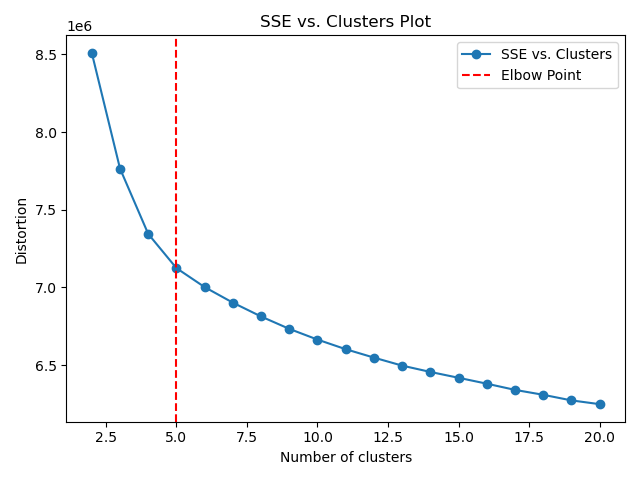
\includegraphics[width=.95\textwidth]{../results/kmeans/SSE_Cluster_Plot.png}
        \caption{SSE vs. No. Clusters}
        \end{subfigure}%
      \begin{subfigure}{.5\textwidth}
        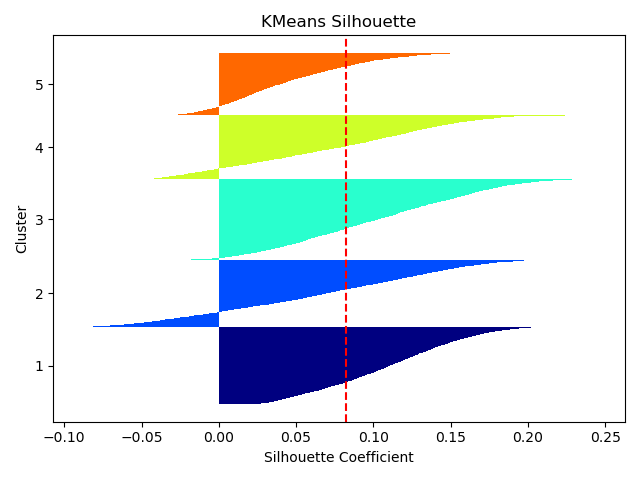
\includegraphics[width=.95\textwidth]{../results/kmeans/Silhouette_Plot.png}
        \caption{Silhouette Plot}
      \end{subfigure}
      \caption{Kmeans Part a}
      \label{figure1}
\end{figure}

\subsection{Part b:}
For problem 1b, we were tasked with generating the Silhouette plot for the optimal choice of clusters. This plot is 
shown in the second part of Figure \ref{figure1}. In this plot we can see that cluster number 1 performed the very 
best, with no elements past 0. However, we can still see that the overall average Silhouette score is quite low, 
clocking in at less than .10 with  some clusters (cluster 2 in particular) showing non-trivial amounts of negative
values.

\subsection{Part c:}
For problem 1c, we were tasked with finding images at the core of their clusters and on the edge of their clusters.
To find the images at the core of their clusters, I took the top 5 highest scoring sample from each cluster. To find
the images at the edge of their clusters, I took the bottom 2 lowest absolute value samples from each cluster.
I chose the minimum absolute value, because if I took the minimum overall then I would get samples which were most 
likely miss-clustered by a large margin, and actually is much closer to another cluster than to it's own cluster. By taking the items who are 
closest to 0, then that point is actually equidistant from each cluster in question which is more closely aligned to 
the definition of being a bordering point. All clusters
except for number 1 had members very close to 0, but cluster 1 had it's lowest members hovering around .2 which was orders
of magnitude higher than the other clusters. Given that behavior, I decided to not include cluster 1 results in the analysis 
of the edge cases given the stipulation of the assignment to only include border cases if they exist.

Looking at the images at the center of clusters, it's clear that the clusters are boats, cars, birds, horses, and planes, 
respectively. This will be important to keep in mind as we analyze the images at the edge of clusters in Figure \ref{figure3}.
Interestingly, we can see that there are 2 nearly identical samples in the plane cluster. I say nearly, because they 
do cluster slightly differently, but it is clear that it is the same image. Regardless, we can pick up on a few consistent 
themes in the center of clusters. And that is: Planes tend to be in the sky and have both wings visible. Boats tend to be 
in the water and also include the skyline, where they likely cover up the transition. Cars are more often bright colors 
and presented in a 3-quarters turned angle. Horses are usually in a clear ground area and broadside. Finally, birds are 
often completely covered in grass and similar coloration to the world around them.


Right away in cluster 2 (cars), we can see that these images are predominantly green and sky blue, respectively. I think that these
backgrounds biased the values to appear more like horses and planes than they would normally seem. Additionally, the car
on the right is a metallic color, which is unlike other cars in its class that are usually painted but more typical of 
planes. I think it is reasonable that these images are bordering two clusters, even though they were correctly clustered.

In cluster 3 (birds), we can see that the image of an ostrich was barely clustered with the birds. I think this is a 
totally fair way to treat the ostrich. If there were any creature I'd put on the border of birds and horses, it would be 
the ostrich. The next image on the border is a car which was incorrectly clustered as a bird, but notably it's the first 
image of a car I've come across which is both facing directly into the camera, and has a door open. Additionally, this 
car is in a field and does not have colors which are not readily found in nature. With these facts in mind, I think that 
this picture is likely reasonable for miss-clustering, but would warrant an analysis of the feature space to understand
what features exactly caused this error.

In cluster 4 (horses), we can see that the first image has a smaller horse which is the darkest color in the image, along
with having it's tail up. Additionally, the front legs are a bit blurred, which causes the image to evoke a similar shape 
and coloration to a rooster nearby a barn. I think that these factors caused this image to be placed on the edge of the 
horse cluster. The right image of the horse cluster is what I believe to be the most intriguing image in this analysis.
This image appears to clearly be a horse, and the only features I can find that could cause it to struggle are the 
inclusion of the person, and the tri-layer background of alternating light-green-dark that was also present in the left 
horse image. 

Finally, in cluster 5 (planes), we can see that the first image is of a plane taken at the same altitude as plane. This 
angle only leaves the tail fin and the cockpit as defining features, and most importantly removes any information 
about the plane's wings. I think that perfectly symmetric wings angled towards a point is likely one of the key differentiating features of 
a plane vs. a boat, given their similar blue shifted backgrounds lacking foliage. On the right image we see a duck 
resting in choppy water. Most importantly, we can see the ducks reflection in the water, which is giving it a symmetric shape
(the heads) angled towards a point (the tail). I think this symmetry along with the cloud-colored water is what caused this 
image to be clusterd on the edge of the plane cluster.


\begin{figure}
    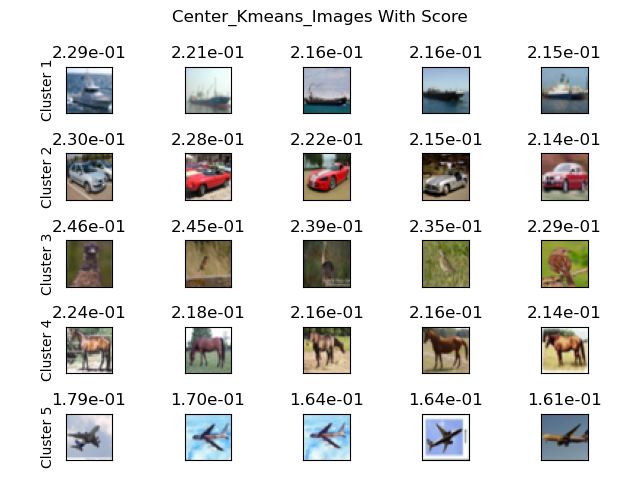
\includegraphics{../results/kmeans/Center_Kmeans_images.png}
    \caption{Images at the Center of Clusters Kmeans}
    \label{figure2}
\end{figure}
\begin{figure}
    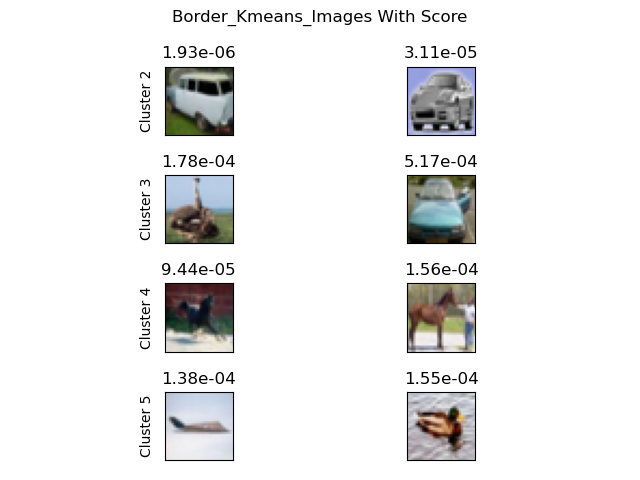
\includegraphics{../results/kmeans/Border_Kmeans_images.png}
    \caption{Images at the Edge of Clusters Kmeans}
    \label{figure3}
\end{figure}

\section{Problem 2:}
\subsection{Part a:}
When it came time to analyze the dendrogram to select the optimal amount of clusters, it was difficult to remove my 
inherent bias towards selecting 5 clusters. Given the fact that the KMeans gave 5 clusters and the ground truth had 5 
classes I had strong prompting to select 5 clusters again. But I wanted to look at this through an objective lens and 
find a feature of the dendrogram which could justify my choice. 

After spending some time looking at Figure \ref{figure4}, I realized that visually the optimal choice of 5 clusters 
minimized the ratio of the variance of the cluster distance over the average cluster distance weighted by the inverse
of the number of
clusters. This is my first interaction with a dendrogram for picking number of clusters, so I was unable to develop and 
test an automated function which matches my hypothesis, and I could not find online others who may have calculated this 
in the same way. Likely, the fact that this method is not easily findable online means that my hypothesis is flawed and
may be overly influence by the behavior of this toy dataset which is well-balanced. Regardless, it is the reasoning which 
I found to best capture why I believe the dendrogram shows 5 clusters to be the optimal number of clusters for the ward method.
\begin{figure}
    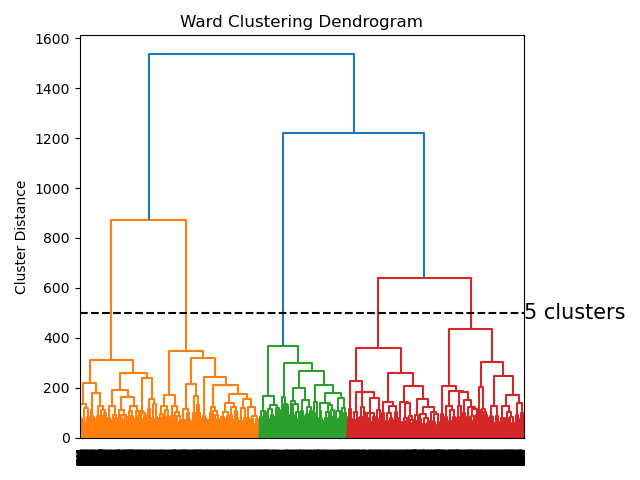
\includegraphics{../results/agglo/Warddendrogram.png}
    \caption{Ward Dendrogram}
    \label{figure4}
\end{figure}

\subsection{Part b:}
The Silhouette plot for the ward method is in Figure \ref{figure5}. This figure is evidence that the agglomerative method
may not be better than the KMeans algorithm for this dataset. Previously, the clusters showed far fewer amounts of points
with a negative Silhouette score, even at a similar overall average score. More in-depth discussion is to follow in part c:
\begin{figure}
    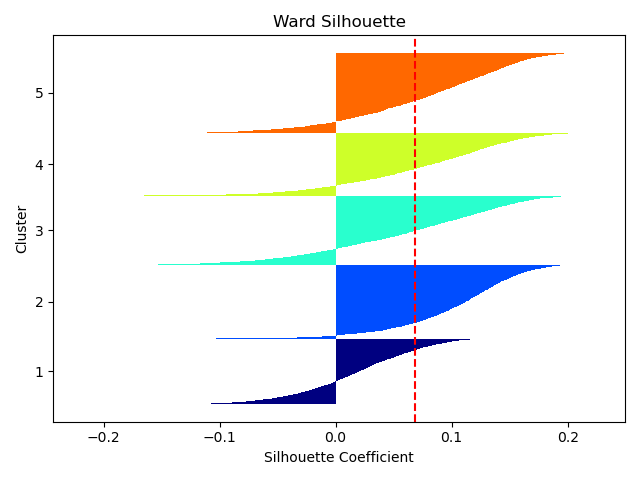
\includegraphics{../results/agglo/Silhouette_Plot_ward.png}
    \caption{Ward Silhouette}
    \label{figure5}
\end{figure}

\subsection{Part c:}
The repeated plots of parts a and b for single linkage and complete linkage are shown in figures \ref{figure6} and \ref{figure7}, 
respectively.

Starting off with the odd one out, the single linkage clustering algorithm appears to have completely missed the mark. 
It seems to have piece-by-piece grown one cluster a single sample at a time until it encompassed the whole group. This 
plot and it's accompanying Silhouette plot show beyond a shadow of a doubt that single linkage is not the direction 
to go with this data. Even when I forced the number of clusters to be 5, the single linkage clustering method caused 
every item to be placed in one group, and no items to be placed in any other clusters leaving 4 empty clusters.

Next, the complete clustering algorithm appears much more reasonable. In an attempt to be fair, I am going to try and 
eyeball my same reasoning I used before. Looking around the line provided in the image, we can see that it appears like 
6 clusters are the optimal number of clusters for this algorithm. However, we can also see that the variance between
the clusters (and cluster balance, but that must imply a balanced dataset) is much worse than the ward algorithm managed.
in the Silhouette plot, we can see that cluster 5 is nothing but an extremely tiny sliver, and should likely be merged
in with another cluster.
\begin{figure}
    \begin{subfigure}{.5\textwidth}
        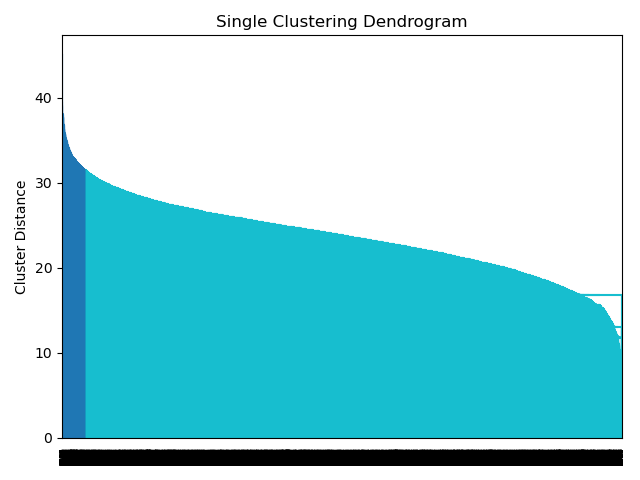
\includegraphics[width=.95\textwidth]{../results/agglo/Singledendrogram.png}
        \caption{Single Dendrogram}
        \end{subfigure}%
      \begin{subfigure}{.5\textwidth}
        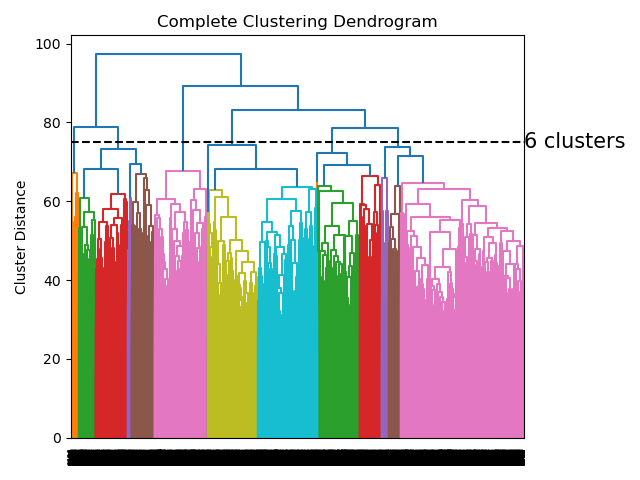
\includegraphics[width=.95\textwidth]{../results/agglo/Completedendrogram.png}
        \caption{Complete Dendrogram}
      \end{subfigure}
\caption{Single and Complete Dendrograms}
\label{figure6}
\end{figure}
\begin{figure}
    \begin{subfigure}{.5\textwidth}
        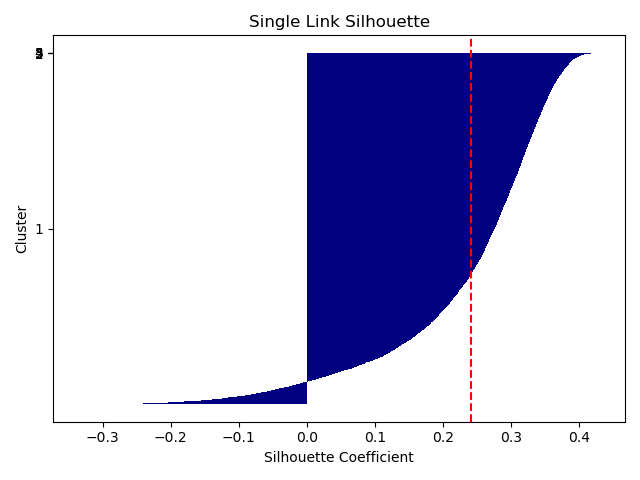
\includegraphics[width=.95\textwidth]{../results/agglo/Silhouette_Plot_single.png}
        \caption{Single Silhouette}
        \end{subfigure}%
      \begin{subfigure}{.5\textwidth}
        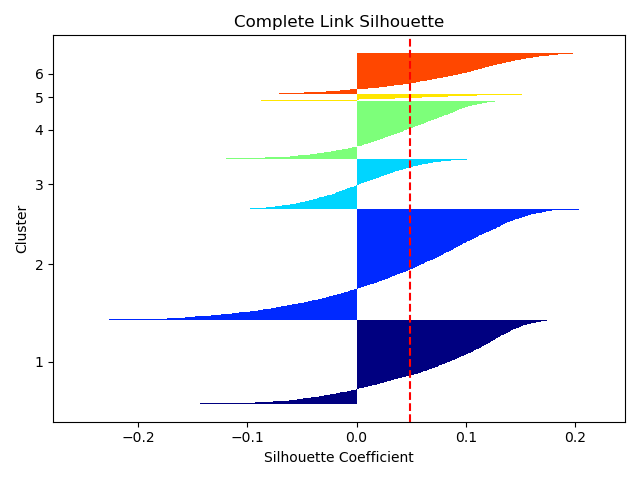
\includegraphics[width=.95\textwidth]{../results/agglo/Silhouette_Plot_complete.png}
        \caption{Complete Silhouette}
      \end{subfigure}
  \caption{Single and Complete Silhouettes}
\label{figure7}
\end{figure}

Looking at the Silhouette plots for all 3 options, I have to stand by the ward algorithm. The clusters created by the
ward distance metric creates more evenly spread clusters with tighter cluster distances between them than the complete 
linkage distance, and the single linkage is practically useless.

\subsection{Part d:}
After picking the Ward algorithm with 5 clusters, I used the same code as before to produce images of samples at the center 
of these clusters and at the edges of these clusters. The images chosen from the centers are actually all nearly identical 
to those chosen in the KMeans. Out of the 25 images presented, only 5 images are different.
As such, most patterns that we can identify are similar to what we had in the KMeans.

Moving on to the items at the edge of the clusters, we actually had representatives of every cluster. Where previously the 
Cluster representing boats had nothing at the edge, we now do have items on the boarder of that cluster.

Cluster 1 (Planes): On the first image, we can see a car which has a single raised part in the center, possibly looking 
like a tail fin. Additionally, the car is not a bright color, but rather a classic color for planes. I think this should 
have definitely been classified with cars, and the fact that it wasn't is concerning. Next, we have a duck in flight. This 
image looks odd to me, like it has some kind of painting vignette around the edges of it. I'm not sure why this image has
those things. I'm certain that they contributed to the missclustering because they could show up similarly to clouds in 
the sky. I think this was clustered as a plane because the background looks more similar to a high-altitude image, and 
the body of the bird is a white color and has clearly visible wings.

Cluster 2 (Boats): I believe the first image is actually an image of two planes overlapping, which is giving an unusual 
outline. I would even hazard to say that this image appears similarly to common erroneous GAN generated images. Furthermore,
the color of the background has a greenish tint which is more commonly associated with maritime photos. Given this, I think
it's understandable that this image was miss-clustered. The second image appears to be of a bird floating on water, but 
the bird takes up a small amount of the image and does not have much detail. Furthermore, it has a color which is commonly
found on boats. I think this is also a reasonable mistake, but still a mistake.

Cluster 3 (Cars): The first image of the car cluster appears to be an older picture, which has a significant amount of
washed-out coloration and out-dated coloration of the car itself. I think that this image is likely unlike the others purely
for the image quality issues, as that will have a significant impact on the similarity between it and other samples. 
The next image is of a dark car on grass only. I think the background and coloration of the vehicle are large drivers for 
this to be on the border. 

Cluster 4 (Horses): The first image is quite hard to make out even for a human. But I believe it to be a pony with 
someone on its back, walking by a strangely colored road. I think the poor resolution of the horse, it's unusual proportions,
and the uniquely striped background likely caused this to be clustered on the edge. Next, we have an image of only a 
horses face next to a human. We've seen enough evidence so far to conclude that likely the clustering algorithm has 
strongly identified the Silhouette of a horse as a driving factor for clustering. This image lacks that information, 
relying almost solely on the coloration. Luckily, the background does contain the natural greenery we often see with 
horse images, and the images poor resolution has caused woman's coloration to be similar to that of a bright grassy
background, such as in column 4 of cluster 4 in the center-clustered images. I think these features saved what would have
been an otherwise very difficult image.

Cluster 5 (Birds): The bird in first image has coloration that is more common in man-made items that we've seen, and additionally
the background is quite blue. Combined together, these features likely caused this image to be pushed more to the edge of 
the bird cluster, even though a classifier would likely classify this as a bird with high certainty. Finally, we see a 
bird flying over reflective water. We saw a similar item previously, where a bird on water that had a reflection made 
clustering difficult, but luckily this time there is separation between the reflection and the bird. I think this made the 
image be clustered at the edge of the cluster, but still able to be clustered correctly.


\begin{figure}
  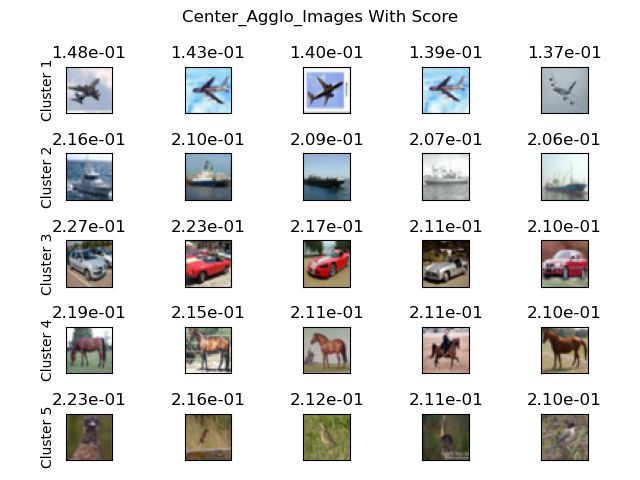
\includegraphics{../results/agglo/Center_Agglo_images.png}
  \caption{Images at the Center of Clusters Agglomerative}
  \label{figure8}
\end{figure}
\begin{figure}
  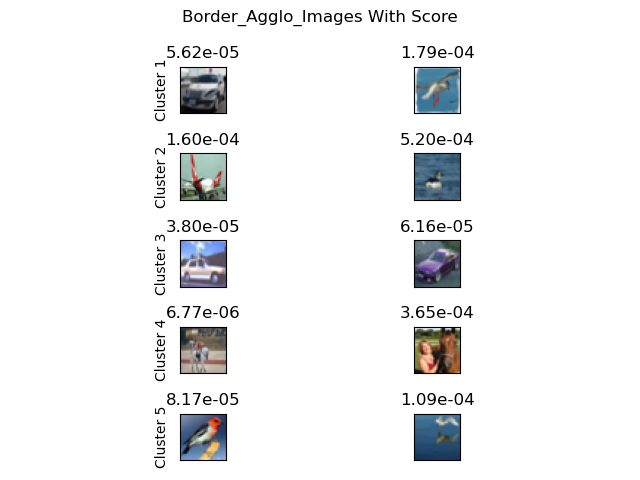
\includegraphics{../results/agglo/Border_Agglo_images.png}
  \caption{Images at the Edge of Clusters Agglomerative}
  \label{figure9}
\end{figure}

\section{Conclusion}
The Kmeans algorithm seems to be better than the Agglomerative algorithm for clustering this data given what we've 
seen so far. The Silhouette plots appeared better. The edge images showed less "Incorrectly" clusterd items. And one 
cluster even had no items significantly close to 0 Silhouette score. Given this evidence, lets look at the ARI values for
each method as a final piece of evidence.

The ARI for the Kmeans and the agglomerative clustering methods are .77 and .69 respectively. I think this is the final 
nail in the coffin for this discussion. The Kmeans is easier to understand and explain to clients, produces more evenly 
split clusters, has better Silhouette scores, accurately predicted the number of classes programmatically, and had 
better Adjusted Rand Index score by a noticeable margin. 

\end{document}